%%%%%%%%%%%%%%%%%%%%%%%%%%%%%%%%%%%%%%%%%
% University/School Laboratory Report
% LaTeX Template
% Version 3.1 (25/3/14)
%
% This template has been downloaded from:
% http://www.LaTeXTemplates.com
%
% Original author:
% Linux and Unix Users Group at Virginia Tech Wiki
% (https://vtluug.org/wiki/Example_LaTeX_chem_lab_report)
%
% License:
% CC BY-NC-SA 3.0 (http://creativecommons.org/licenses/by-nc-sa/3.0/)
%
%%%%%%%%%%%%%%%%%%%%%%%%%%%%%%%%%%%%%%%%%

%----------------------------------------------------------------------------------------
%	PACKAGES AND DOCUMENT CONFIGURATIONS
%----------------------------------------------------------------------------------------

\documentclass{article}

\usepackage{graphicx} % Required for the inclusion of images
\usepackage{natbib} % Required to change bibliography style to APA
\usepackage{amsmath} % Required for some math elements
\usepackage{mathtools}
\usepackage[export]{adjustbox}
\usepackage{subcaption}
\usepackage{float}
\usepackage{listings}
\usepackage{minted}

\DeclarePairedDelimiter{\abs}{\lvert}{\rvert}
\setlength\parindent{0pt} % Removes all indentation from paragraphs

\renewcommand{\labelenumi}{\alph{enumi}.} % Make numbering in the enumerate environment by letter rather than number (e.g. section 6)

%\usepackage{times} % Uncomment to use the Times New Roman font

%----------------------------------------------------------------------------------------
%	DOCUMENT INFORMATION
%----------------------------------------------------------------------------------------

\title{ECE 637 Digital Image Processing Laboratory: \\ Eigen-decompostion of
Images} % Title

\author{Yang \textsc{Wang}} % Author name

\date{\today} % Date for the report

\begin{document}

\maketitle % Insert the title, author and date

%----------------------------------------------------------------------------------------
%	SECTION 1
%----------------------------------------------------------------------------------------

\section{Introduction}
	Nothing due for report.

%----------------------------------------------------------------------------------------
%	SECTION 2
%----------------------------------------------------------------------------------------
\section{Multivariate Gaussian Distributions and Whitening}
	\subsection{Generating Gaussian Random Vectors}
	\begin{figure}[h]
		\begin{center}
		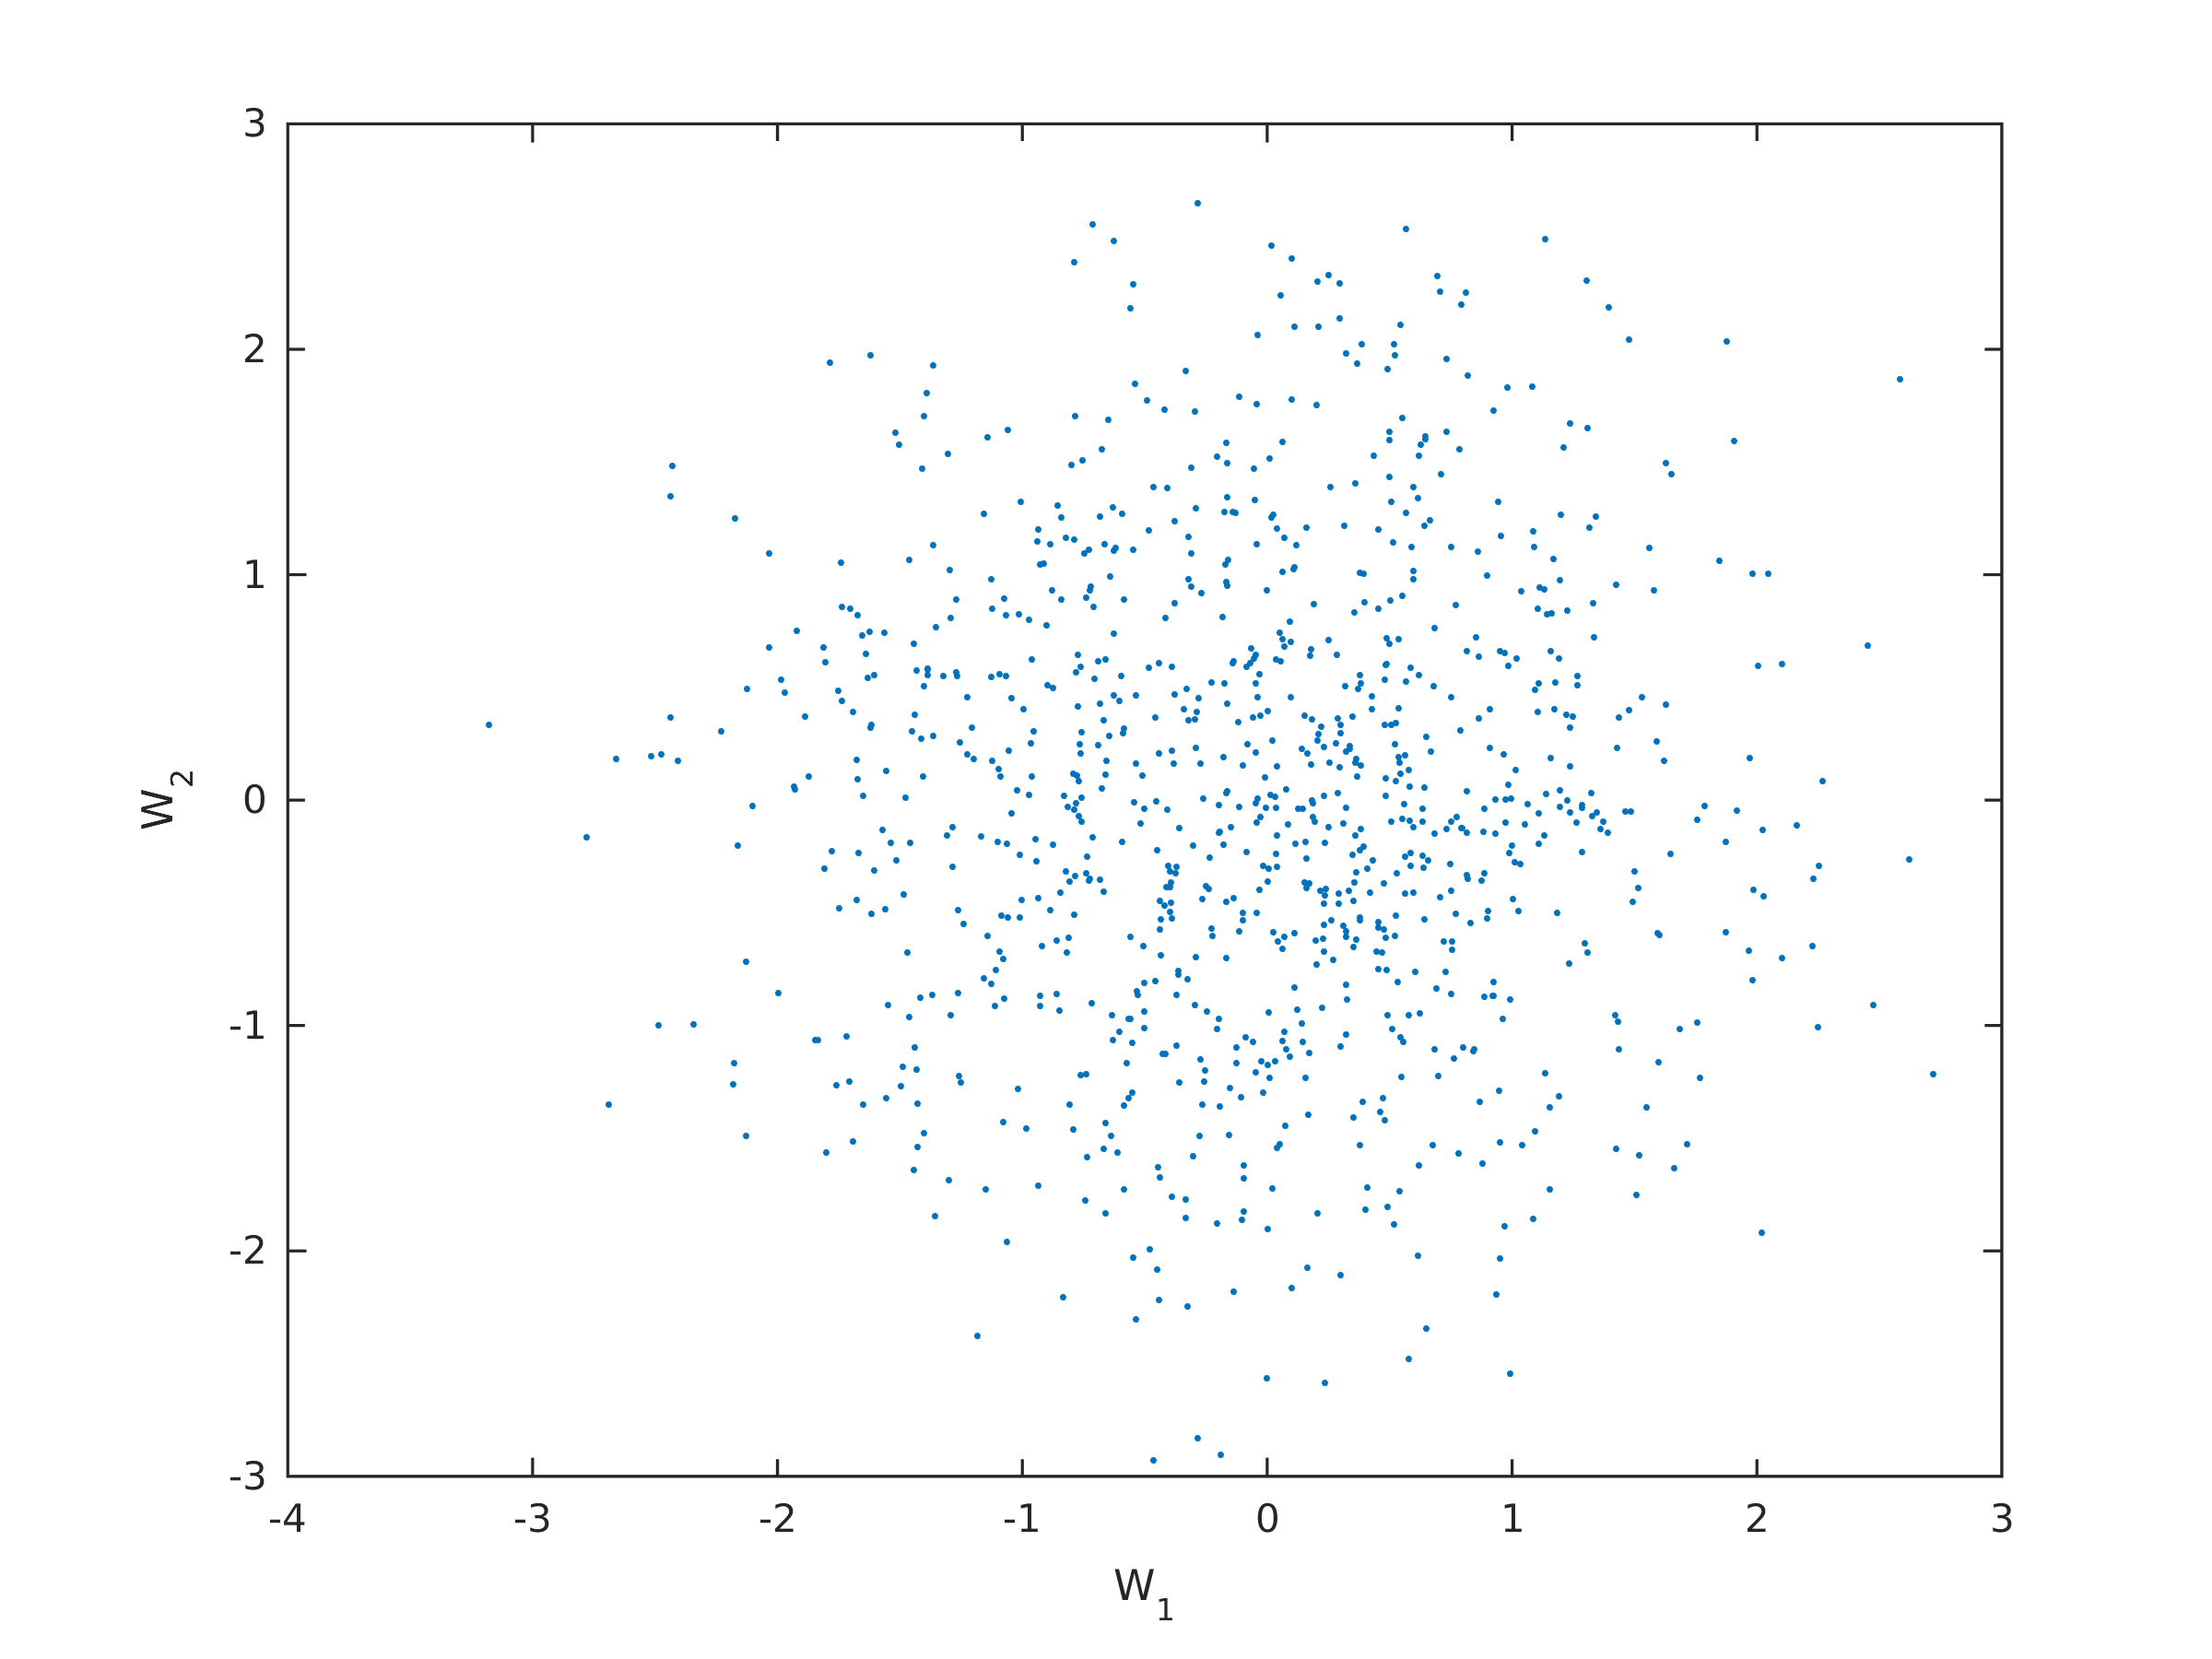
\includegraphics[width=0.75\textwidth]{rvW.png}
		\caption{Scatter plot for $W$}
		\end{center}
	\end{figure}
	\begin{figure}[h]
		\begin{center}
		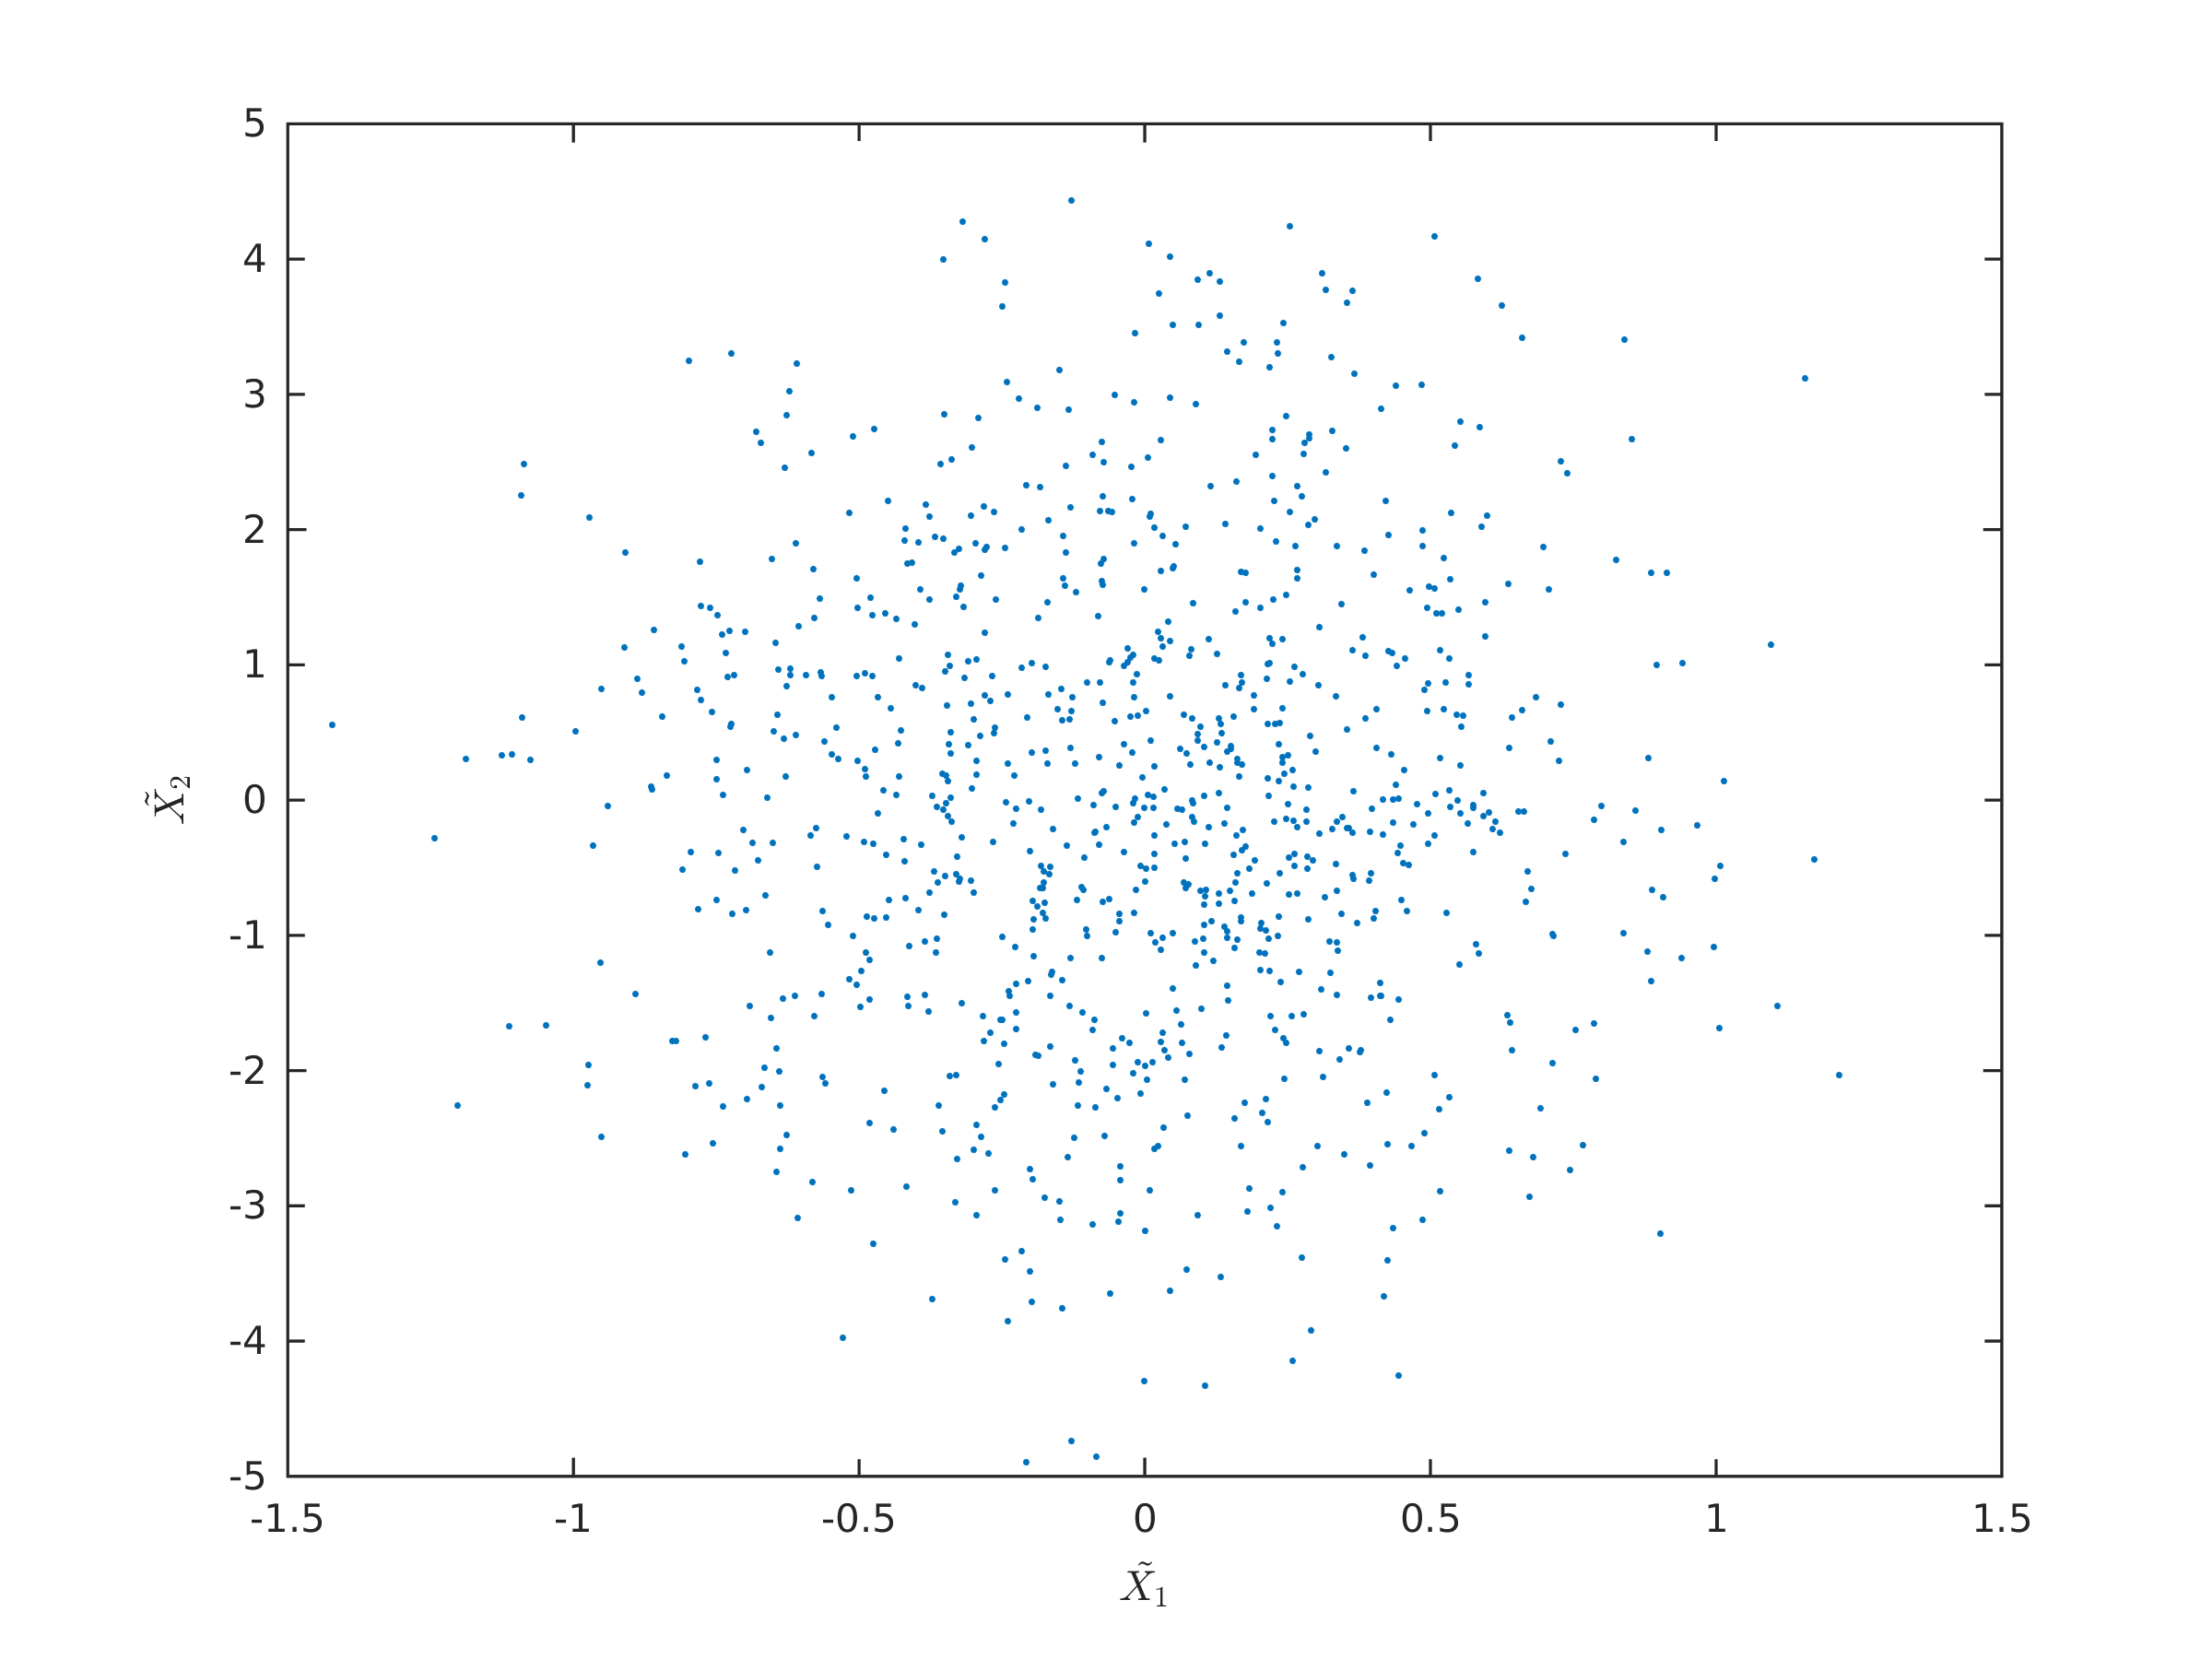
\includegraphics[width=0.75\textwidth]{rvXtilda.png}
		\caption{Scatter plot for $\tilde{X}$}
		\end{center}
	\end{figure}
	\begin{figure}[h]
		\begin{center}
		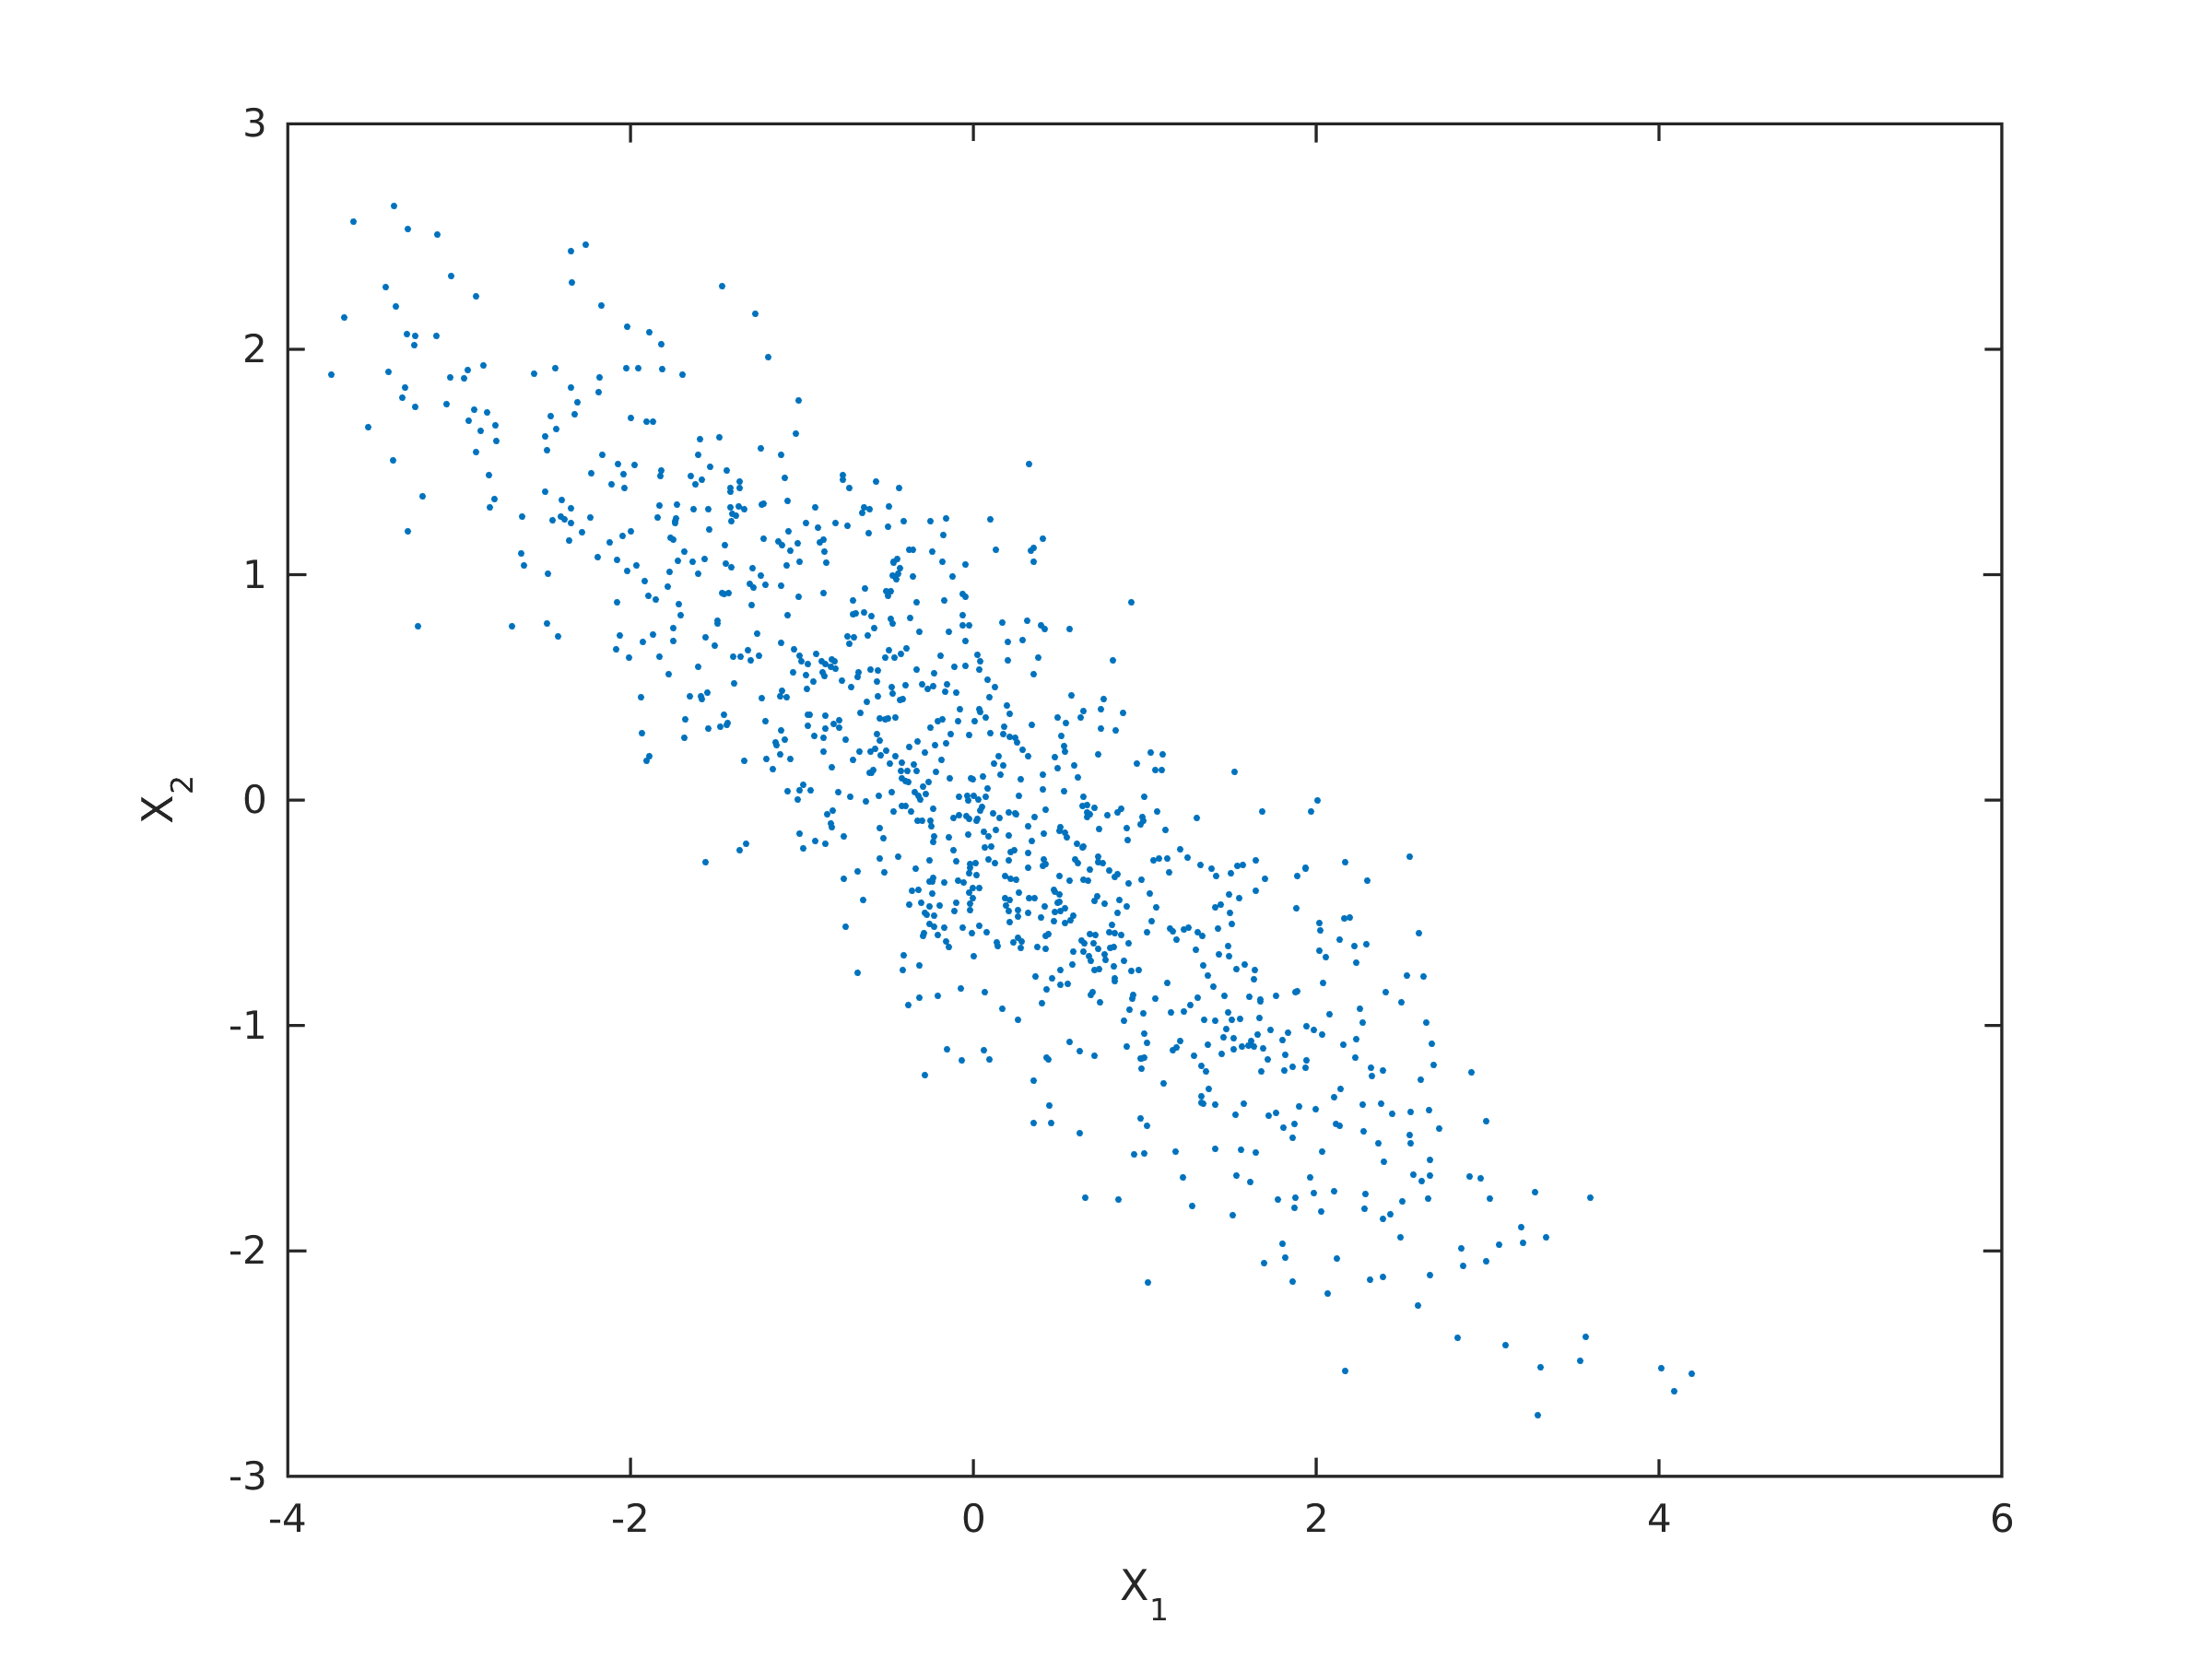
\includegraphics[width=0.75\textwidth]{rvX.png}
		\caption{Scatter plot for $X$}
		\end{center}
	\end{figure}

\pagebreak

	\subsection{Covariance Estimation and Whitening}
		\subsubsection{Theoretical Value of $R_{x}$}
			\begin{align*}
				R_{x} =
				\begin{bmatrix}
					2 & -1.2 \\
					-1.2 & 1
				\end{bmatrix}
			\end{align*}
		\subsubsection{Estimated Value of $\hat{R_{x}}$}
			\begin{align*}
				\hat{R_{x}} =
				\begin{bmatrix}
					2.0383 & -1.2230 \\
					-1.2230 & 1.0133
				\end{bmatrix}
			\end{align*}
		\subsubsection{Scatter Plots for $\tilde{X_{i}}$ and $W_{i}$}
			\begin{figure}[h]
				\begin{center}
				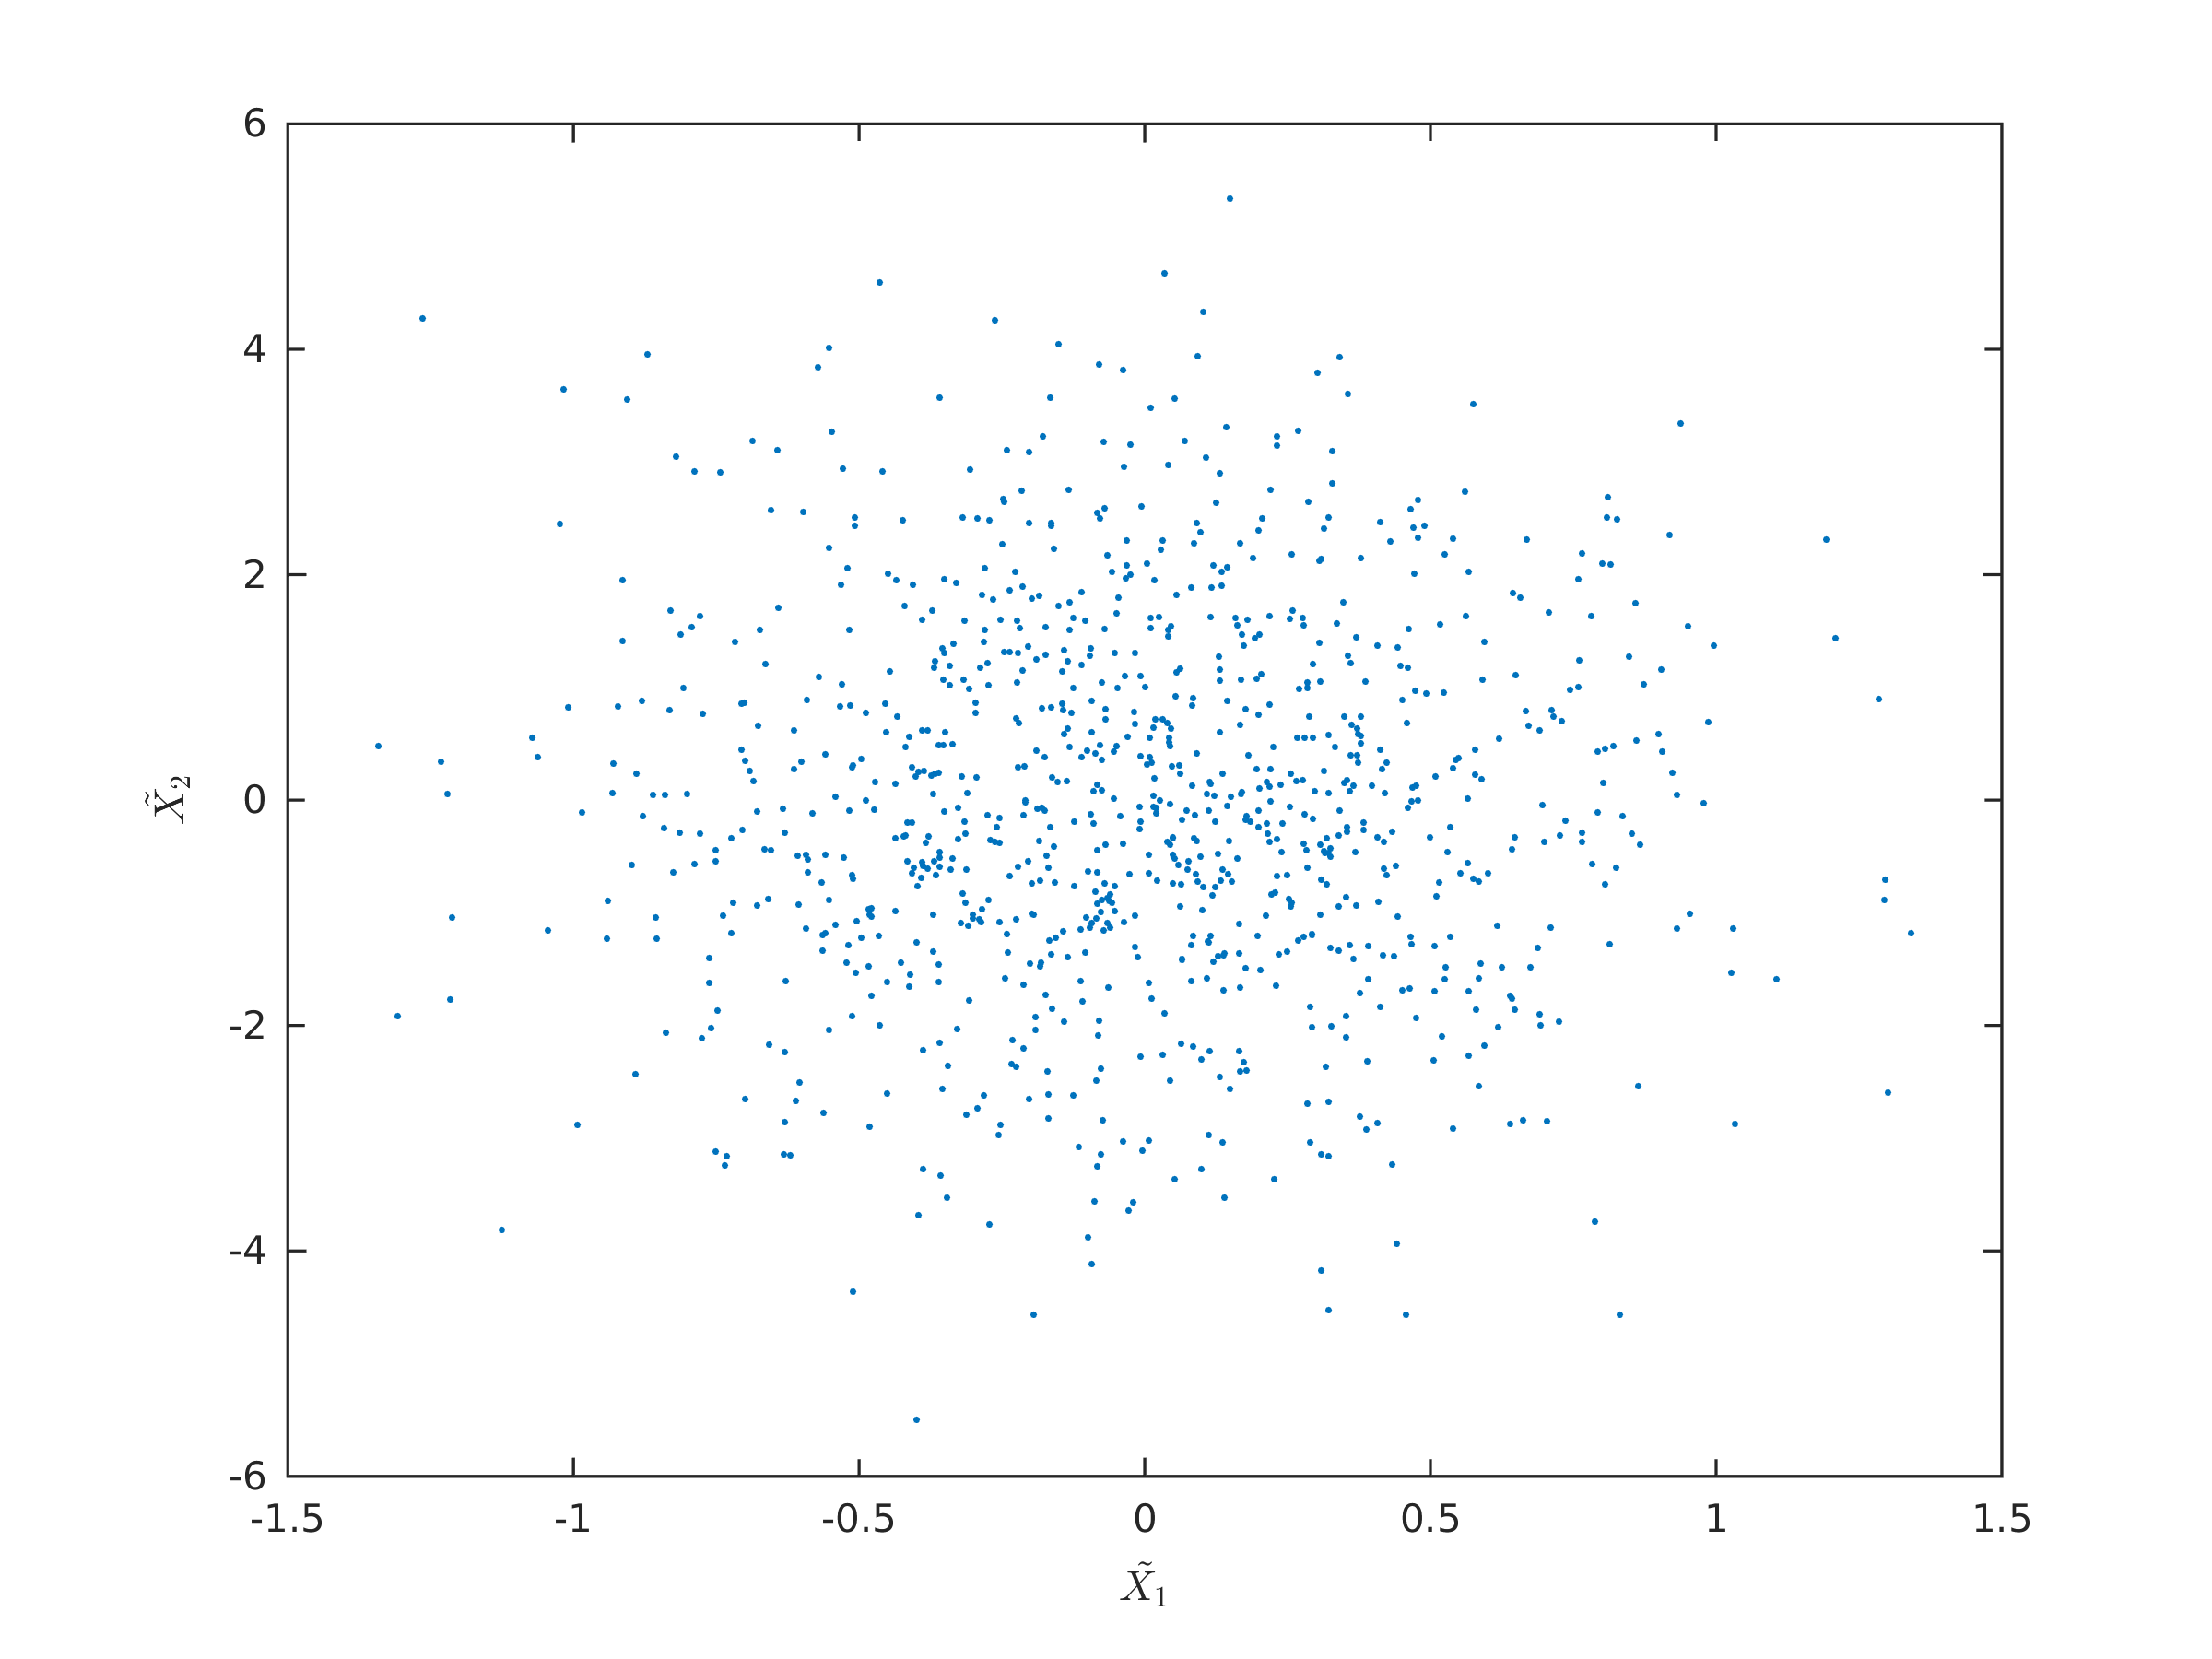
\includegraphics[width=0.75\textwidth]{rvXtildaEsti.png}
				\caption{Scatter plot for $\tilde{X_{i}}$}
				\end{center}
			\end{figure}
			\begin{figure}[h]
				\begin{center}
				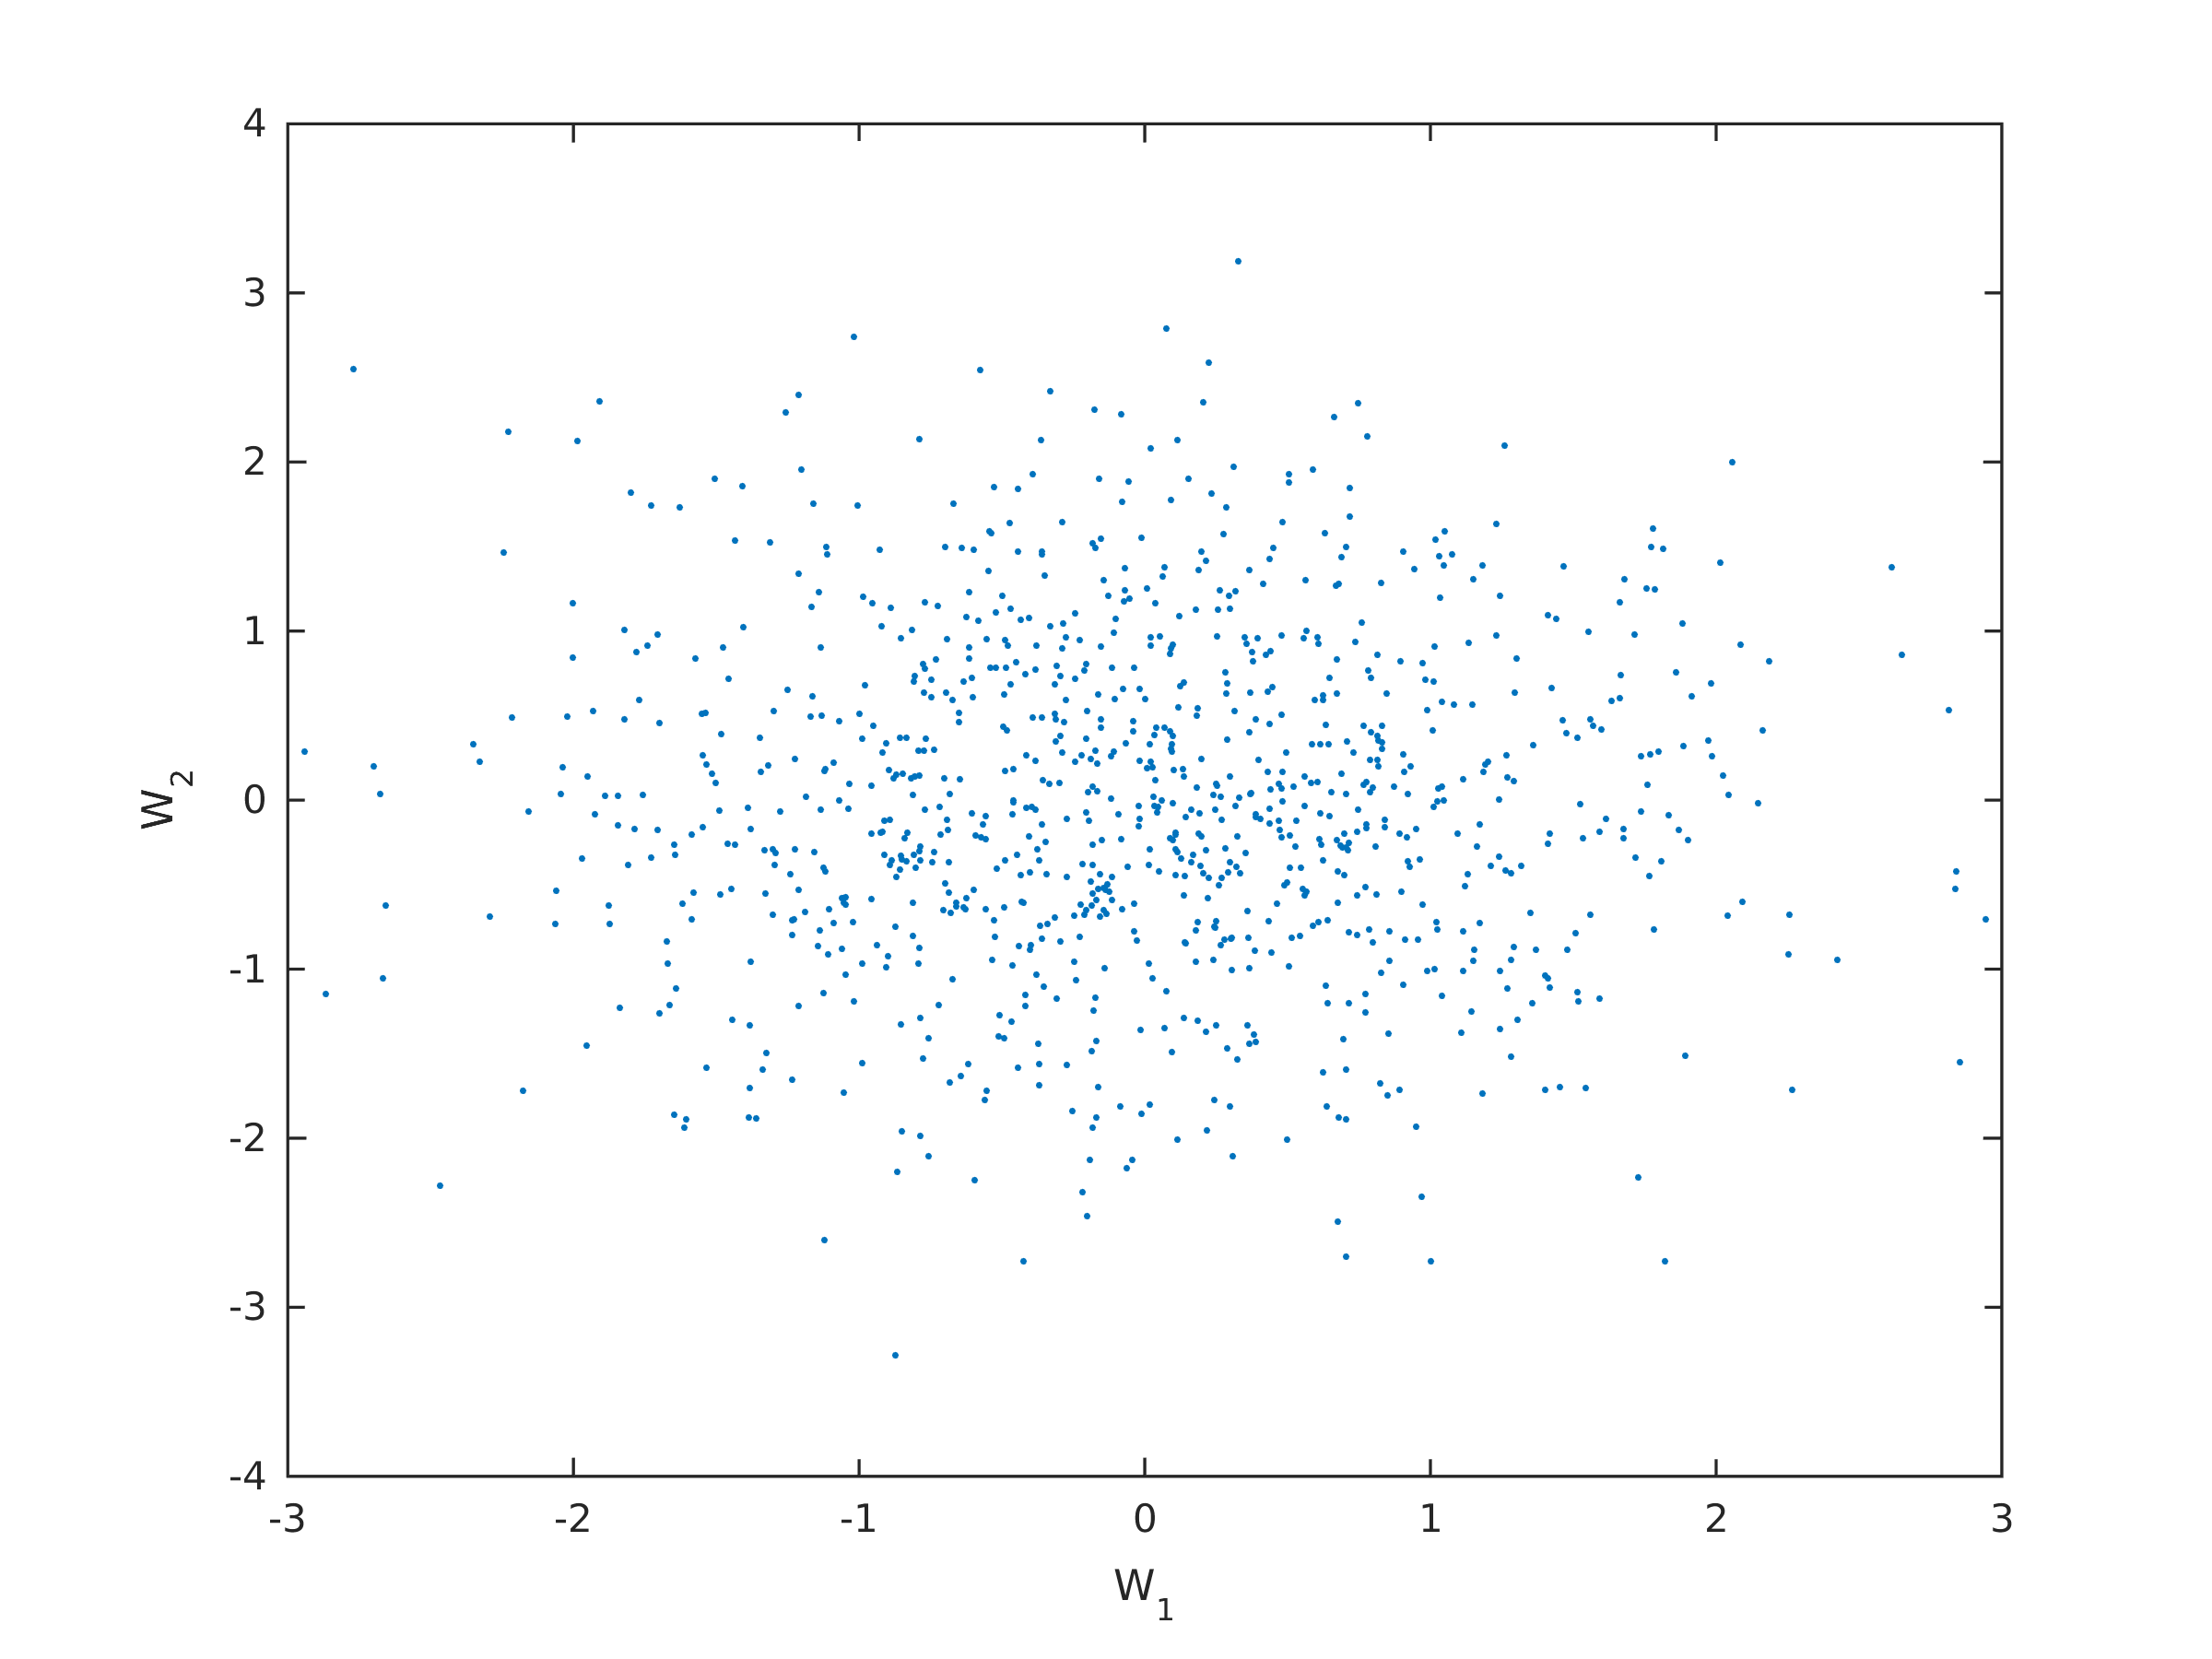
\includegraphics[width=0.75\textwidth]{rvWEsti.png}
				\caption{Scatter plot for $W_{i}$}
				\end{center}
			\end{figure}
		\subsubsection{Estimated Covariance of Whitened Process}
			\begin{align*}
				\hat{R_{W}} =
				\begin{bmatrix}
					1 & 0 \\
					0 & 1
				\end{bmatrix}
			\end{align*}


%----------------------------------------------------------------------------------------
%	SECTION 3
%----------------------------------------------------------------------------------------


%----------------------------------------------------------------------------------------
%	SECTION 4
%----------------------------------------------------------------------------------------

\end{document}
